\documentclass[a4paper, 11pt]{article}
\usepackage[slovene]{babel}
\usepackage{comment} % enables the use of multi-line comments (\ifx \fi) 
\usepackage{lipsum} %This package just generates Lorem Ipsum filler text. 
\usepackage{fullpage} % changes the margin
\usepackage{graphicx}
\usepackage{comment}
\usepackage{url}
\usepackage[utf8]{inputenc}
\usepackage{amsfonts}
\usepackage[dvips]{psfrag}
\usepackage{fancyref}
\usepackage{graphicx}
\usepackage{epsfig}
\usepackage{amsmath}
\usepackage{amssymb}
\usepackage{tikz}
\usepackage{booktabs}
\usepackage{diagbox}
\usepackage{listings}


\graphicspath{{img/}}

\begin{filecontents*}{report.bib}
@MISC{WikipediaEN:IPI,
    author = {{Wikipedia, the free encyclopedia}},
    title = {Incubation preiod},
    year = {2017},
    note = {[Online; dostop 17 Avgust, 2017]},
    url = {https://upload.wikimedia.org/wikipedia/commons/0/04/Concept_of_incubation_period.svg}
}
\end{filecontents*}


\begin{document}
\noindent
\large\textbf{Poročilo o končnem projektu} \hfill \textbf{Filip Koprivec} \\
\normalsize Matematično modeliranje, 2016/2017 \hfill Vpisna številka: 27141059 \\


\section*{Navodila}
S pomočjo metode Monte Carlo analizirajte širjenje nalezljive bolezni na $2d$ mreži. Preverite, kako različni populacijski parametri (precepljenost) vplivajo na širjenje bolezni in končno stanje.

\section*{Uvod}
Nalezljive bolezni so skozi zgodovino človeštva pomembno vplivale na celosten razvoj civilizacije in življenja posameznika. Skozi zgodovino je v kolektivnem spominu ostalo kar nekaj pomembnejših izbruhov nalezljivih bolezni (Črna smrt, ki je konec srednjega veka pomorila med 30 in 60\% evropskega prebivalstva, različne mrzlice, ki so ob prihodu Evropejcev ohromile prebilvastvo Amerik, do Španske gripe, ošpic in drugih.). Epidemije so s spreminjanjem populacijske dinamike pogosto močno spremenile tok zgodovine, bile pa so tudi pomemben razlog, ki je omejeval velikosti mest. Še celo v 19. stoletju sta bila tako London kot Pariz pogosto deležna izbruhov kolere, katerih vzrokov pa vse do razvoja teorije mikroorganizmov kot povzročiteljev bolezni ni bilo mogoče razložiti. V 20. stoletju pa je človeštvo z razvojem antibiotikov in cepiv mnoge izmed bolezni izkoreninili (črne koze, v Zahodnem svetu tudi očpice, rdečke in otroško paralizo).

Cepiva pa poleg odpornosti na bolezen prinašajo tudi stranske učinke, hkrati pa zaradi sestave ne smemo cepiti vseh prebivalcev določenega območja (alergija na učinkovino, alergija na beljakovine v cepivu itd.). Prav tako pa je določen del populacije vedno necepljen (novorojenčki do prejema cepiva, ljudje z osljabljenim imunskim sistemom, ljudje po presaditvi kostnega mozga, itd.). Klub temu pa lahko z dovolj veliko stopnjo precepljenosti vseeno zagotovimo tako imenovano čredno imunost, ko imuni posamezniki preprečujejo prenos bolezni do posameznikov, ki so dovzetni za okužbo. S pomočjo matematičnih modelov lahko tako preučujemo širjenje bolezni v populaciji glede na različne stopnje precepljenosti in pridemo do različnih zaključkov. Eden izmed zaključkov je lahko: pri kakšni stopnji precepljenosti je posamezna okužba (pri ustreznem ravnanju ob odkritju okužbe) omejena na manjše geografsko območje, kdaj pa kljub (sicer premajhnemu) deležu cepljenih pride do epidemije.

\section*{Analiza problema}
\subsection*{Različni modeli}
V projektni nalogi se osredotočimo na poenostavljen problem epidemije v populaciji. Zamislimo si zaprto populacijo (državo), v dovolj kratkem času, da normalni populacijski dejavniki ne pridejo do izraza (smrti, rojstva, emigracija). V veliki večini modeli populacijo razdelijo v več razdelkov. Eden izmed najbolj znanih (zveznih) modelov je tako imenovani SIR model, ki populacijo razdeli v tri dele: \emph{Susceptible} (osebki dovzetni za okužbo - zdravi), \emph{Infected} (okuženi osebki, ki lahko okužijo nove, ozdravijo, ali pa podležejo bolezni) in \emph{Removed} (osebki, ki so iz modela odstranjeni (se ne morejo okužiti), kot posledica smrti, lahko pa tudi kot posledica kakih drugih dejavnikov). Z nekaj malega znanja o biologiji lahko preprosto zapišemo sistem diferencialnih enačb za tak model:
\begin{align*}
	S' &= \Lambda(N) - \beta S I - \mu S \\
	I' &= \beta S I - \mu I -\alpha I  + \alpha I \\
	N' &= \Lambda(N) - (1-f)\alpha I - \mu N 
\end{align*}

Kjer je: $\Lambda(N)$ število rojstev, $\beta$ koeficient infektivnosti, $\mu$ splošna smrtnost, $\alpha$ smrtnost bolezni in $f$ delež osebkov, ki bolezen prebolijo z imunostjo. S pomočjo konstant lahko model kontroliramo. Pri večini modelov nas ne zanima celostna rešitev (ki je analitično navadno ne moremo dobiti), navadno je dovolj, če poznamo stacionarne točke, ter obnašanje v okolici. Vprašanje, ki se ga največkrat vprašamo je: Ali število okuženih hitro raste in so po dovolj dolgem časo okuženi vsi, ali se ustali pri nekem deležu populacije, ali pa bolezen odmre (po nekaj časa).

Naslednji razvoj modela je tako imenovani SIS model, ki bolje upošteva tudi dejstvo, da na nekeatere bolezni pridobimo imunost. Natančenjše analie modela tu ne bomo dodajali, je pa pomemben ker lahko določimo osnovno reprodukcijsko število ($R_0$), ki nam pove, kakšno je obnašanje števila okuženih po dovolj dolgem času.

\subsection*{Naključni model}
V svojem projektu sem si bolj podrobno ogledal simulacijski model. Predpostavimo fiksno število osebkov na 2d mreži, kjer vsakemu osebku priredimo svojo celico. Namesto na razdelkih populacije, simulacija deluje na nivoju posameznika, zato si lahko privoščimo nekoliko preurejen SEIR model, kjer posamezniku priredimo več značilnosti. Te značilnosti so podrobneje opisane tudi v kodi. Posamezniku priredimo več značilnosti, ki so pomembne za kužnost, prenosljivost in smrtnost bolezni:
\begin{enumerate}
\item \textbf{Starostna skupina}: Pomembna je zaradi učinkovitosti cepiv, smrtnosti pri različnih modelih, ter zaradi prenosljivosti. Ob bolj natančni simulaciji (za katero ni niti časa, niti procesorja, niti delovnega spomina), bi lahko s pomočjo starosti nadzorovali infektivnost posameznika zaradi različne razdalije potovanja (vožnja v sližbo), socialne skupine (otroci v šoli ali vrtcu so v stiku z velik drugimi otroci) in imajo v splošnem slabši imunski sistem, spolne aktivnosti, načina življenja, itd.
\begin{enumerate}
\item Otrok: do 14 let
\item Odrasel: od 15 do 64 let
\item Starejši: od 64 let naprej
\end{enumerate}

\item \textbf{Spol}: Spol je pomemben zaradi prenosljivosti različnih bolezni, smrtnosi, pri državah v razvoju tudi zaradi različnih socialnih krogov, ter ob simulacijah spolno prenosljivih bolezni.
\begin{enumerate}
\item Ženski
\item Moški
\end{enumerate}

\item \textbf{Status cepljenja}: S pomočjo bolj natančne razdelitve cepljenja lahko omogočimo simulacije, ki natančneje upoštevajo realno stanje, kjer določen delež cepiv ni učinkovit, ali pa so cepiva že stara, targetirajo drug sev bolezni (cepiva za gripo), ali pa so osebki sveže cepljeni.
\begin{enumerate}
\item Ni cepljen: posameznik ni cepljen, edina zaščita pred boleznijo je čredna imunost
\item Popolnoma cepljen: Posameznik je popolnoma cepljen, cepivo učinkuje, zanj ni verjetnosti da se naleze, saj je odporen na bolezen (dokler ne mutira)
\item Sveže cepljen: Sveže cepivo je navadno manj učinkovito, sa telo še ni povsem pripravljeno
\item Staro cepivo/drug sev: Cepivo je manj učinkovito, saj je staro, ali targetira drug sev bolezni
\item Nedelujoče cepivo: Pri večini cepiv določen delež posameznikov kljub cepljenu ni odporen (cepivo nu učinkovito), to stanje je enako kot Ni cepljen
\end{enumerate}

Poleg fizičnih lastnosti pa posamezniku glede na stanje obolelosti pripada še nekaj drugih značilnosti:

\item \textbf{Stanje infekcije}: V kakšnem stanju je pri posamezniku bolezen. Predvsem pomembna za ugotavljanje trenutnega stanja mreže.
\begin{enumerate}
\item Ni okužen: Posameznik (še) ni (bil) okužen
\item Trenutno okužen: Posameznik je trenutno okužen, simulacija poteka, dokler je vsaj še en posameznik okužen
\item Okužen v preteklosti: Posameznik je bil v preteklosti okužen, a je bolezen uspešno prebolel (lahko so sicer nastale komplikacije, a zaradi bolezni ni umrl). Model v osnovi predpostavi, da s tem posameznik pridobi imunost na nadaljne infekcije.
\item Mrtev: Posameznik je za posledicami bolezni umrl.
\end{enumerate}

\begin{figure}[h]
\caption{Grafični prikaz različnih stanj bolezni na časovni premici. Prevzeto iz \cite{wikiimg}.}
\label{img:incubation}
\centering
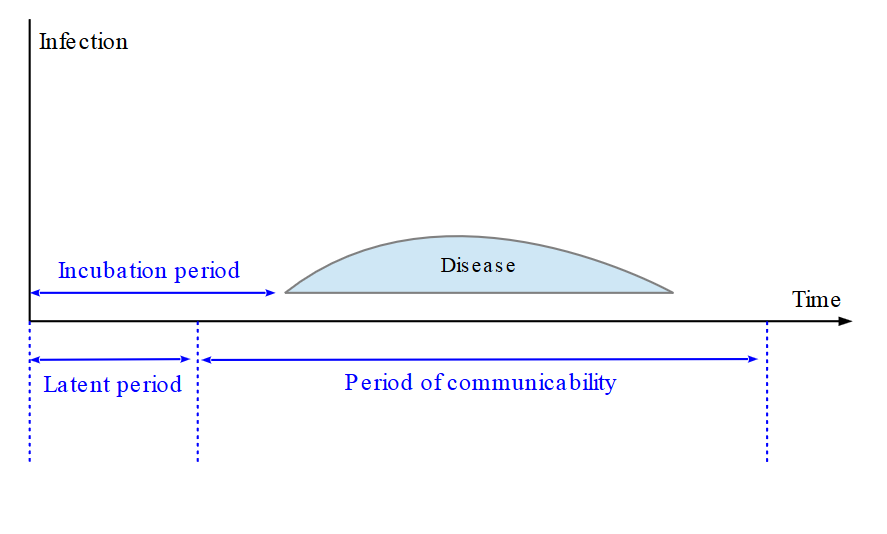
\includegraphics[width=1\textwidth]{incubation_concept.png}
\end{figure}

\item \textbf{Stanje bolezni}: V kakšnem simptomatskem stanju je pri posamezniku bolezen. Kljub temu da je posameznik okužen, je lahko bolezen nevidna (v inkubacijski dobi). Posameznik je sicer okužen, a ne kaže (vidnih) znakov okužbe. Tak posameznik je lahko vseeno kužen četudi ne kaže simptomov.
\begin{enumerate}
\item Inkubacijska doba: Posameznik je z boleznijo okužen, a ne kaže znakov (te se navadno pojavi nekaj dni(ošpice) po okužbi, pri nekaterih bolezni pa lahko to traja tudi več let ali desetletji (HIV, Kuru). 
\item Simptomatska doba: Posameznik je z boleznijo okužen in kaže simptome (fleki na koži, tresoče roke), kljub simpotomom posameznik ni nujno kužen.
\end{enumerate}

\item \textbf{Stanje nalezljivost}: Pove, ali je posameznik kužen ali ni. Odnos med simptomi in kužnostjo najlepše prikaže slika \ref{img:incubation}.
\begin{enumerate}
\item Ni kužen: Posameznik ni kužen
\item Kužen: Posameznik lahko okuži ljudi okoli sebe.
\end{enumerate}

\item \textbf{Trajanje bolezni}: Kako dolgo je posameznik okužen. S pomočjo tega parametra določamo kdaj posameznik postane kužen začne kazati simptome, ozdravi, itd. Ob vsakem koraku iteracije modela se ta parameter poveča za $1$ in se ustrezno posodobijo njegova stanja.

\item \textbf{Dotaknjen}: Parameter je uporabljen za spremljanje poti epidemije. Vsakič ko posameznik pride v stik z okuženim (bi se potencialno lahko okužil) posameznik postane dotaknjen. S tem lahko spremljamo razširjenost epidemije in njeno napredovanje, ter možne varne točke. Take posameznike označimo za prizadete s strani bolezni, saj so bili v stiku z okuženimi.

\end{enumerate}

Za primerno spremljanje infekcije poleg podatkov o posamezniku potrebujemo tudi osnovne parametre bolezni, te so:
\begin{enumerate}
\item \textbf{Dolžina inkubacijske dobe}
\item \textbf{Čas trajanja simptomatske bolezni}
\item \textbf{Dolžina latentnega obdobja}
\item \textbf{Čas trajanja infektivnosti posameznika}
\item \textbf{Smrtnost bolezni}: Delež okužeih, ki v času okužbe umre. Za potrebe simulacije predpostavimo, da je bolezen smrtna zgolj v simptomatski fazi. Nadalje predpostavimo, da je smrtnost vsak dan enako verjetna in neodvisna. Iz tega izračunamo \textbf{verjetnost smrti} (mortality\textunderscore rate), ki ga uporabimo pri koraku simulacije.
\item \textbf{Infektivnost bolezni}: Ta parameter je najtežje ugotoviti iz biološko/medicinskega opisa bolezni. Za njegov pomen sem vzel verjetnost, da se po preteku infektivnega obdobja posameznik v kontaku za kužnim okoži. Iz tega podobno kot pri smrtnosti ob predpostavki o enakomernosti in neodvisnosti izpeljemo \textbf{verjetnost infekcije}.
\item \textbf{Razdalija nalezljivosti} Parameter ki pove, kako daleč se bolezen lahko razširi. Po analogiji je blizu vrsti prenosa bolezni in z njim modeliramo različne oblike prenoslijvosti. Kapljično ali po zraku prenosljive bolezni imajo večjo razdalijo, medtem ko bolezni, ki se prenašajo zgolj z dotikom simuliramo z manjšimi števili. Kombinacija infektivnosti in razdalije nalezljivosti nam tako povesta kako hitro oziroma daleč se bolezen širi.
\end{enumerate}

Celotna simulacija epidemije poteka na kvadratni 2d mreži, ki jo zaradi smiselnosti 'ovijemo' z vseh strani. Formalno: identificiramo nasprotni si stranici na mreži in dobimo nekakšno sfero. Še bolj formalno: uvedemo ekvivalčno relacijo med točkami na mreži s predpisom: 
$$(x,y) \cong (x',y') \iff x-x' = w*k \land y-y' = h*l; k,l \in \mathbb{N}$$
kjer je $w$ širina mreže in $h$ višina mreže. S tem dosežemo, da je stanje na mreži odvisno zgolj od relativne postavitve posameznikov in lahko za najlepši pregled nad širjenjem epidemije začetnega okuženega postavimo kar na sredino mreže.

\section*{Delovanje programa}
Program deluje kot preprosta simulacija. V vsakem koraku simuliramo časovno enoto 
%NEMA PREDAJE:4.22
 med epidemijo. Na začetku si glede na starostno in spolno strukturo države generiramo kvadratno mrežo (brez težav bi lahko generirali tudi poljubno pravokotno), ki jo v programu predstavimo kot gnezden seznam objektov Person. Vsaki osebu glede na podatke o državi priredimo tudi stanje cepiva. Za začetek simulacije okužimo poljubno osebo(ali več), navadno na sredini zaradi lažjega spremljanja okužbe. Stopnjo cepljenosti lahko posplošimo in jo razumemo kot splošno (prirojeno ali pridobljeno) odpornost na bolezen. Skozi zgodovino lahko tako odpornost opazimo z nihanjem smrtnosti pri ponovni epidemiji v kratkem času (Kuga se je v Evropi pojavila še večkrat, a z mnogo manjšim učinkom kot v prvi epidemiji).

\subsection*{Korak simulacije}
V vsakem koraku simulaicje se po vrsti (vrstni red sicer ni pomemben) sprehodimo po mreži in vsakemu okuženemu posamezniku povečamo število dni okužbe in ustrezno posodobimo stanja (stanje okužbe in infektivnosti). Če posameznik kaže simptome, potem z verjetnostjo, ki jo določuje bolezen v simulaciji umre. Posameznik, ki je v nekem koraku umrl lahko še vedno okuži druge (kužna so tudi trupla, vse skupaj pa utemeljimo z dejstvom, da se smrti 'dogajajo' samo na koncu koraka). Če je posameznik kužen, potem poljubnega posameznika, ki je na mreži oddaljen manj kot razdalija kužnosti (popravljena glede na število ljudi v celici, v osnovi uporabljamo $d_1$ metriko, bolj znano kot Manhattansko ali taksi razdalijo) izvedemo funkcijo okužanja. Funkcija okužanja posameznika ki ni okužen z določeno verjetnostjo okuži, pri tem pa upošteva stanje cepljenja (cepljenje popolnoma onemogoči okužbo, medtem ko stara in sveža cepiva zgolj zmanjšajo verjetnost). Če se okuži nov posameznik si to zapomnimo in na koncu ustrezno posodobimo mrežo. Po končanem koraku vrnemo objekt, ki vsebuje trenutne spremembe na mreži in podatke o trenutnem stanju mreže.

% to comment sections out, use the command \ifx and \fi. Use this technique when writing your pre lab. For example, to comment something out I would do:
%  \ifx
%	\begin{itemize}
%		\item item1
%		\item item2
%	\end{itemize}	
%  \fi

\section*{Opazovanje rezultatov}
Simulacije bolezni z različnimi stopnjami precepljenosti bomo obravnavali na podoben način kot pri zveznih primerih opisanih iz uvoda, hkrati pa poskušali ugotovitve razložiti z zgodovinskega in geografskega vidika. V osnovi lahko razvoj bolezni razdelimo na dve veliki skupini. V prvi skupini se bolezen začne na nekem ozkem območju in se razširi v epidemijo, kjer zajame celotno mrežo. Zgodovinski primer tega so znane epidemije: Črna smrt, Španska gripa, nalezljive bolezni v Ameriki s prihodom Evropejcev, epidemija sifilisa v Evropi, \dots V drugem primeru paokužba ostane omejena na manjšem območju (mesto, vas), kjer se večina populacije okuži, a se bolezen zaradi različnih razlogov ne razširi drugam. To je lahko posledica manjšega potovanja, slabe povezanosti med mesti (večina epidemij se je v zgodovini zgodila na višku razcveta trgovine), imunosti okolice (so že preboleli okužbo), ali pa karantene. Med različnimi simulacijami bom primerjal, kako stopnja precepljenosti vpliva na končo stanje (epidemija ali lokalni izbruh). Iz analitične izpeljave sledi, da je meja dokaj ostra (ob upoštevanju da lahko rezultati zaradi uporabe simulacije variirajo).

\section*{Analiza in razultati}
Vse simulacije sem izvajal na prednastavljeni mreži, ki predstavlja Slovenijo (z 10 ljudmi v posamezni celici), s spremenljivo stopnjo precepljenosti. Za bolezen sem vzel prednastavljeno bolezen ošpic. Vse simulacije so bile opravljene na sistemu Windows 10, 64bitnem procesorju in 32bitnem Pythonu 3.6 (Natančneje: Python 3.6.0 (v3.6.0:41df79263a11, Dec 23 2016, 07:18:10) [MSC v.1900 32 bit (Intel)] on win32)

\subsection*{Primerna precepljenost}
V Sloveniji se po priporočilih NIJZ priporoča 95 odstotna precepljenost, da okužba ne izbruhne (realna precepljenost je nekoliko nižja). Rezultati simulacije s takimi parametri so prikazani v tabeli \ref{tab:full_vaccination}. Vidimo da je okuiženih zelo malo, saj se okužba ne 'prenese' prek precepljenih. Rezultati sicer malo skačejo, a okužba je zadržana na zelo majhnem območju in do epidemije ni prišlo. Jasno se vidi tako imenovana čredna imunost, ko večina necepljenih ljudi kljub dejstvu, da niso imuniziriani ni bila okužena, saj niso prišli v stik z okuženimi. Bolj podrobno poročilo, ki ga zgenerira glavni program za naključno seme 2017 je vidno na sliki \ref{img:2017_ful_vac}. Jasno je vidno, da najprej število okuženih naraste, nato pa bolezen izumre.

\begin{figure}[h]
\caption{Podrobno poročilo, ki ga pripravi program za stopnjo precepljenosti 95\%}
\label{img:2017_ful_vac}
\centering
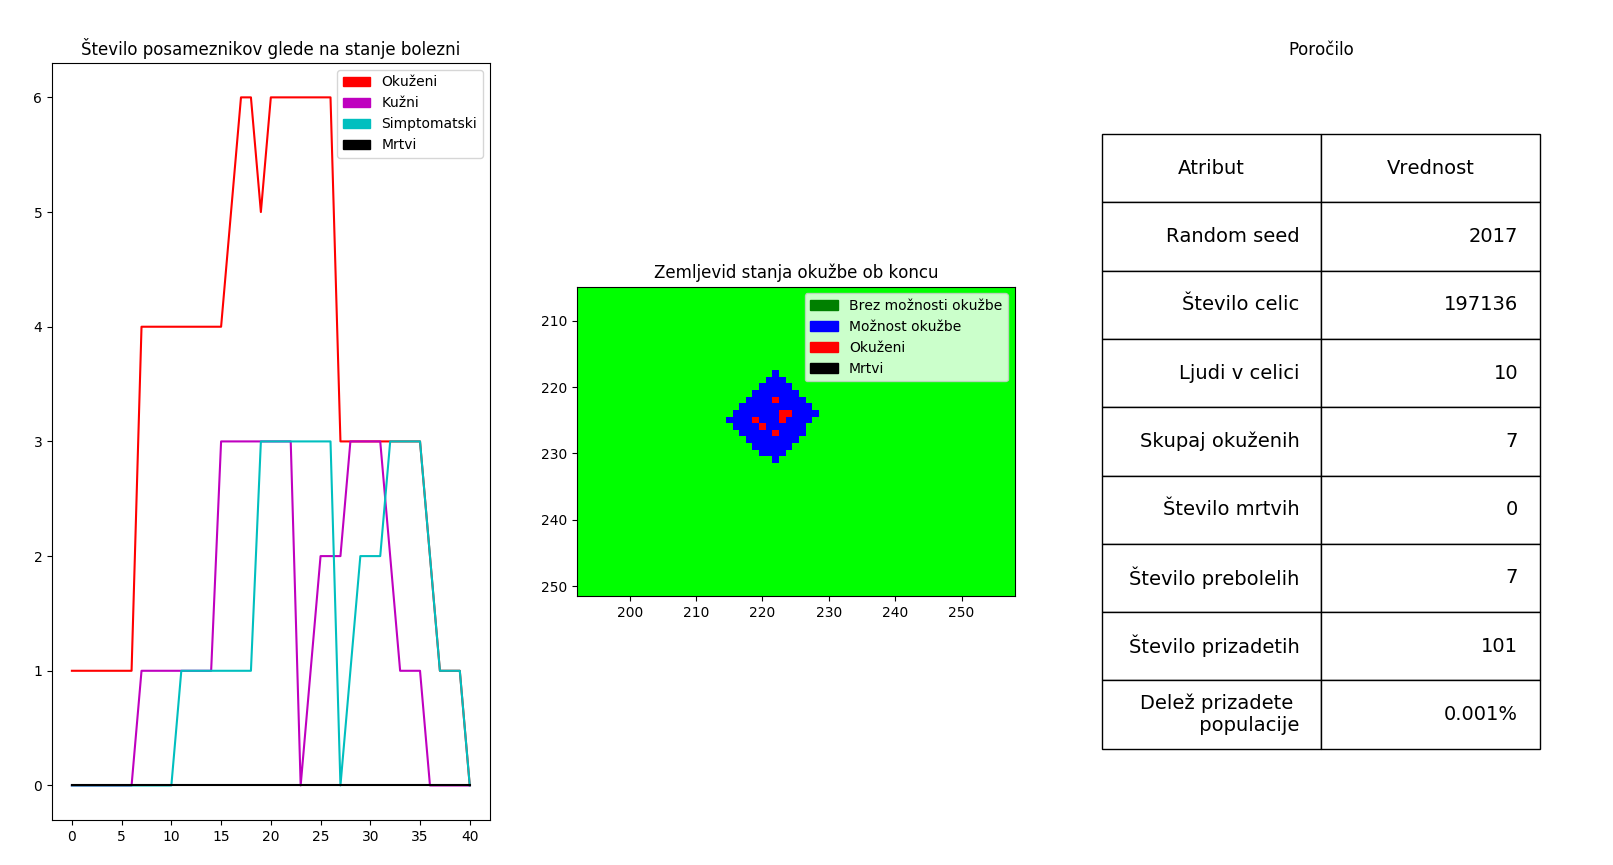
\includegraphics[width=1\textwidth]{2017_ful_vac.png}
\end{figure}


\begin{table}[h]
\centering
\caption{Rezultati simulacije pri 95\% precepljenosti}
\label{tab:full_vaccination}
\begin{tabular}{|l||l|l|l|l|}
\hline
\backslashbox{seed}{atributi} & Število okuženih & Število mrtvih & Delež prizadete populacije \\ \hline \hline
1992 & 1 & 0 & 0.000\% \\ \hline
1994 & 1 & 0 & 0.000\% \\ \hline
1996 & 5 & 0 & 0.000\% \\ \hline
1998 & 2 & 0 & 0.000\% \\ \hline
2000 & 5 & 0 & 0.000\% \\ \hline
\end{tabular}
\end{table}

Če pa precepljenost spustimo na 85\%, dobimo rezultate prikazane v tabeli \ref{tab:not_full_vaccination}. Jasno vidimo, da nastane epidemija, saj se bolezen ne zadrži na mestu. Bolj natančno poročilo pri semenu 2017 vidimo na sliki \ref{img:2017_not_ful_vac}. Vidimo, da je bolezen zajela celotno področje. Obolelih sicer ni veliko, saj je stopnja precepljenosti še vedno kar visoka, vendar je bolezen dosegla skoraj vse, ki niso bili cepljeni. Ta simulacija (in vse ostale z nižjo stopnjo precepljenosti) dobro pokažejo, kako pomembna je čredna imunost za zaščito tistih, ki se ne morejo cepiti. Če si pogledamo graf števila okuženih posameznikov lahko opazimo manjše vrhove, ki se pogosto pojavljajo v epidemijah. Še bolj zanimiva stvar pa so zeleni 'otoki' na mreži, ki prikazujejo območja, ki se jih bolezen ni dotaknila. Ker je stopnja precepljenosti ravno pod mejo za epidemijo, je bolezen zajela večino prebivalstva, del pa je bil vseeno uspešno obkrožen z imunimi osebki, kar ga je izoliralo. Tudi ta pojav ima zgodovinski in realni analog, saj so znani primeri, ko so se posamezne vasi zgolj s pomočjo 'sreče' izognile sicer smrtni okužbi.

\begin{figure}[h]
\caption{Podrobno poročilo, ki ga pripravi program za stopnjo precepljenosti 85\%}
\label{img:2017_not_ful_vac}
\centering
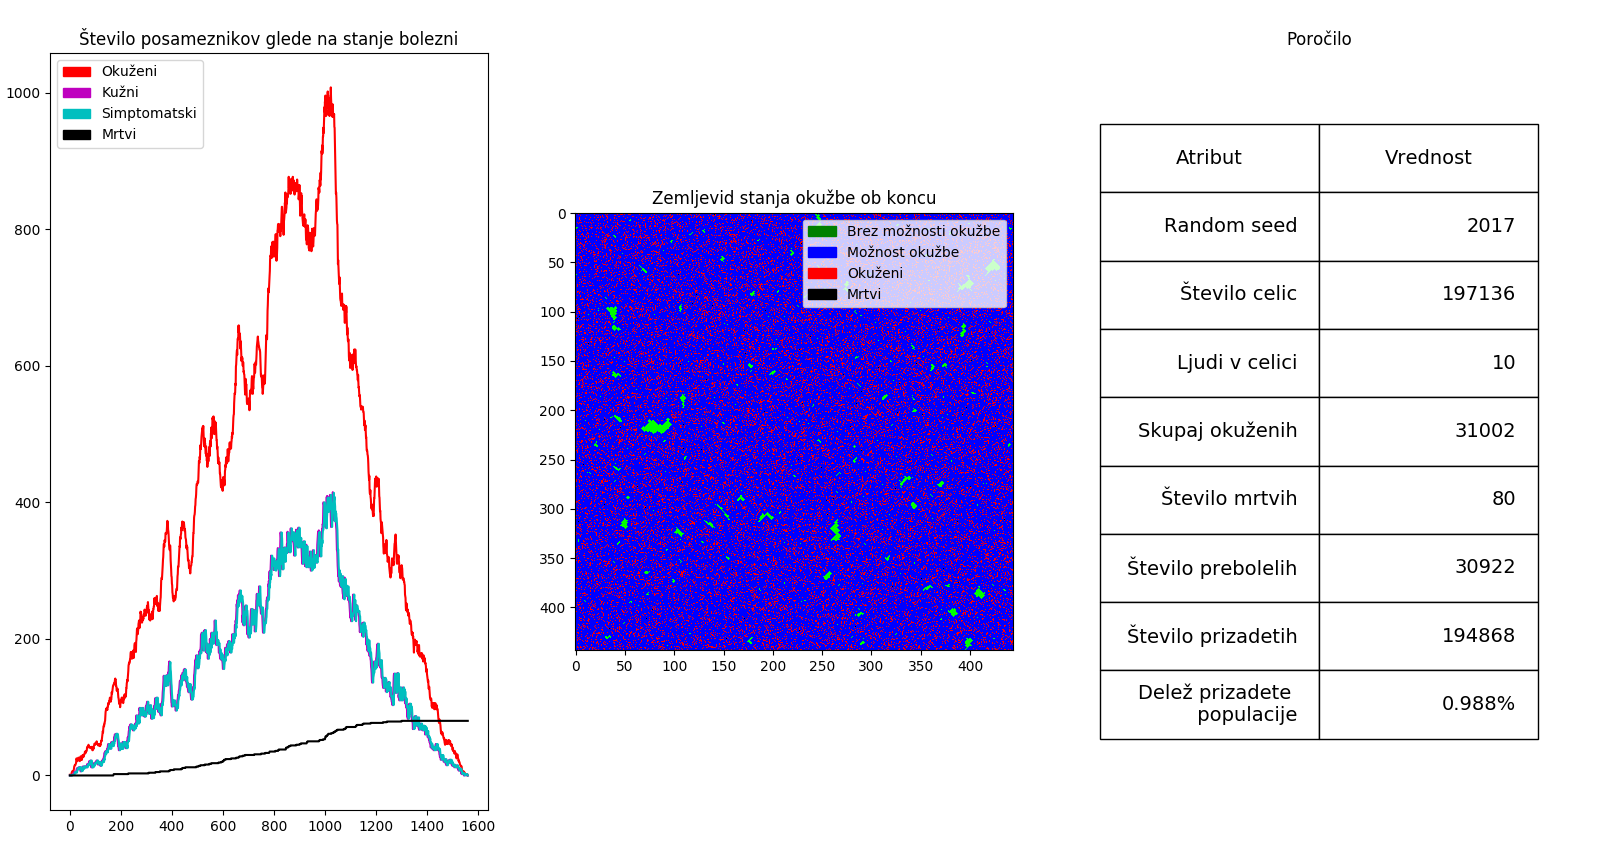
\includegraphics[width=1\textwidth]{2017_not_ful_vac.png}
\end{figure}

\begin{table}[h]
\centering
\caption{Rezultati simulacije pri 85\% precepljenosti}
\label{tab:not_full_vaccination}
\begin{tabular}{|l||l|l|l|l|}
\hline
\backslashbox{seed}{atributi} & Število okuženih & Število mrtvih & Delež prizadete populacije \\ \hline \hline
1992 & 31300 & 88 & 0.988\% \\ \hline
1994 & 31279 & 71 & 0.991\% \\ \hline
1996 & 30261 & 84 & 0.979\% \\ \hline
1998 & 30945 & 78 & 0.992\% \\ \hline
2000 & 31283 & 81 & 0.992\% \\ \hline
\end{tabular}
\end{table}

\section*{Zaključek}
Zaključki simulacij, ki jih opravi program se večina skladajo z začetnimi opazovanji širjenj bolezni v zgodovini. Če v programu vklopimo sprotni prikaz širjenja bolezni lahko opazujemo širjenje, ki se zdi konsistentno s predpostavkami modela (okužba se širi enakomerno v vse smeri).

Seveda ima model kar nekaj slabosti. Prva je predpostavka o konstantnem kontaktu med ljudi. Posameznikom bi lahko priredili parameter premikanja, s katerim bi lahko kontrolirali širjenje. Po drugi strani pa bi s tem model postal veliko bolj nepredvidljiv, saj bi v slučaju da se okuži človek, ki veliko potuje močno spremeni končno situacijo modela. Model prav tako predpostavi konstantno nalezljivost in umrljivost, kar ni nujno res. Pomembna pomankljivost modela je neodzivnost človeške populacije na bolezen. V realnem življenju se okolica hitro odzove na pojav bolezni. Prav tako je v takem modelu težko nadzorovati dejstvo, da okuženi potujejo manj in zmanjšajo stike z drugimi, hkrati pa tega pojava ni opaziti v času ko se simptomi ne kažejo, oseba pa je kužna.

Možna izboljšava bi bila kombinacija zveznega in simulativnega modela, kjer bi namesto fiksnih celic z zveznim modelom modelirali manjše koščke mreže, ki bi jih potem uporabili naprej v simulaciji.

\section*{Uporaba programa}
Program je napisan in preizkušen v programskem jeziku Python verzije 3.6, najverjetneje pa deluje tudi v verziji 3.5 (V nižjih verzijah bi bilo za delovanje potrebno odstraniti označbe tipov). 

Pred zagonom je potrebno namestiti zahtevane pakete. Za namestitev priporočam uporaba virtualnega okolja (virtualenv). Potrebne pakete namestimo z ukazom:
\noindent See the following command :
\begin{lstlisting}[language=bash]
  $ pip install -r requirements.txt
\end{lstlisting}

Ko so potrebni paketi nameščeni preprosto s poženemo datoteko main.py, ki glede na nastavitve (opisane v programu s komentarji) začne simulacijo in prikaže rezultate.




\begin{thebibliography}{9}
\bibitem{math_models} BRAUER, Fred, in, CASTILLIO-CHÁVEZ, Carlos Castillo-Chávez \emph{Mathematical Models in Population Biology and Epidemiology}. New York: Springer-Verlag. ISBN: 978-1-4419-3182-5
\bibitem{Math_epidem}  BRAUER, Fred, et al. \emph{Mathematical Epidemilogy}. Heidelberg: Springer-Verlag. ISBN: 978-3-540-78910-9
\bibitem{articles} FENG, Zhilan, et al. \emph{Disease Evolution: Models, Concepts, and Data Analyses}. ISBN:0-8218-3753-2

\bibitem{wikiimg} Wikipedia, the free encyclopedia. Incubation period, 2017. URL https://upload.wikimedia.org/wikipedia/commons/0/04/Concept\textunderscore of\textunderscore incubation\textunderscore period.svg [Online; Datum dostopa 17. Avgust, 2017]
\end{thebibliography}


\hfill \textit{Filip Koprivec}


\end{document}
